\section{Baza danych}
\begin{figure}
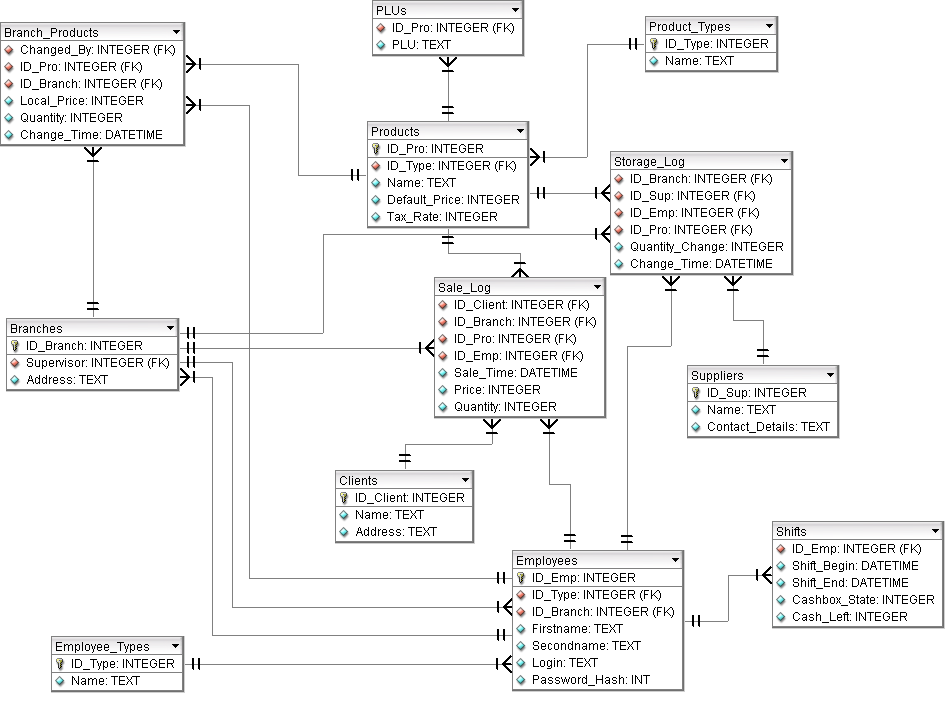
\includegraphics[width=1\textwidth]{gfx/baza.png}
\caption{Schemat bazy danych}
\end{figure}
Opis tabel:
\begin{description}
\item[Branches] każdy rekord tabeli odpowiada jednemu salonowi
    \begin{description}
    \item[ID\_Branch] - identyfikator salonu (klucz główny)
    \item[Supervisor] - identyfikator kierownika salonu (klucz obcy do tabeli Employees)
    \item[Address] - adres salonu
    \end{description}
\item[Employees] dane pracowników
    \begin{description}
    \item[ID\_Emp] - identyfikator pracownika (klucz główny)
    \item[ID\_Branch] - identyfikator salonu, w którym pracuje dany pracownik (klucz obcy do tabeli Branches)
    \item[Firstname] - imię pracownika
    \item[Secondname] - nazwisko pracownika
    \item[Login] - nazwa pracownika w systemie
    \item[Password\_Hash] - skrót kryptograficzny hasła pracownika
    \end{description}
\item[Shifts] zmiany pracowników
    \begin{description}
    \item[ID\_Emp] - pracownik, którego dotyczy dana informacja o zmianie (klucz obcy do tabeli Employees)
    \item[Shift\_Begin] - czas rozpoczęcia zmiany
    \item[Shift\_End] - czas zakończenia zmiany
    \item[Cashbox\_State] - stan kasy na zakończenie zmiany
    \item[Cash\_Left] - wartość zasiłku pozostawionego kolejnej zmianie
    \end{description}
\item[Products] dane dotyczące produktów
    \begin{description}
    \item[ID\_Pro] - identyfikator produktu (klucz główny)
    \item[ID\_Type] - typ produktu (klucz obcy do tabeli Product\_Types)
    \item[Name] - nazwa produktu
    \item[Default\_Price] - domyślna cena produktu
    \item[Tax\_Rate] - wartość podatku, jakim objęty jest produkt
    \end{description}
\item[Branch\_Products] dane dotyczące produktów, w konkretnych salonach
    \begin{description}
    \item[Changed\_By] - pracownik, wprowadzający zmianę (klucz obcy do tabeli Employees)
    \item[ID\_Pro] - identyfikator produktu (klucz obcy do tabeli Products)
    \item[ID\_Branch] - identyfikator salonu (klucz obcy do tabeli Branches)
    \item[Local\_Price] - cena produktu w salonie
    \item[Quantity] - ilość produktu dostępnego w salonie
    \end{description}
\item[Sale\_Log] dziennik sprzedaży
    \begin{description}
    \item[ID\_Client] - identyfikator klienta otrzymującego fakturę lub NULL, jeżeli faktura nie została wydana (klucz obcy do tabeli Clients)
    \item[ID\_Branch] - salon, w którym nastąpiła sprzedaż (klucz obcy do tabeli Branches)
    \item[ID\_Pro] - sprzedawany produkt (klucz obcy do tabeli Products)
    \item[ID\_Emp] - pracownik odpowiedzialny za sprzedaż (klucz obcy do tabeli Employees)
    \item[Sale\_Time] - czas sprzedaży
    \item[Price] - cena
    \item[Quantity] - ilość
    \end{description}
\item[Storage\_Log] dziennik operacji na magazynie
    \begin{description}
    \item[ID\_Branch] - salon, którego dotyczy operacja (klucz obcy do tabeli Branches)
    \item[ID\_Sup] - identyfikator dostawcy (klucz obcy do tabeli Suppliers)
    \item[ID\_Emp] - pracownik odpowiedzialny za operację (klucz obcy do tabeli Employees)
    \item[ID\_Pro] - produkt, którego dotyczy operacja (klucz obcy do tabeli Products)
    \item[Quantity\_Change] - zmiana ilości stanu magazynu, wartość dodatnia oznacza przyjęcie towaru, ujemna --- wydanie
    \item[Change\_Time] - czas wykonania operacji
    \end{description}
\item[Product\_Types] typy produktów
    \begin{description}
    \item[ID\_Type] - identyfikator typu (klucz główny)
    \item[Name] - nazwa typu
    \end{description}
\item[Suppliers] dane dostawców
    \begin{description}
    \item[ID\_Sup] - identyfikator dostawcy (klucz główny)
    \item[Name] - nazwa dostawcy
    \item[Contact\_Details] - szczegóły dotyczące kontaktu z dostawcą
    \end{description}
\item[Clients] dane klientów (do faktur)
    \begin{description}
    \item[ID\_Client] - identyfikator klienta (klucz główny)
    \item[Name] - nazwa klienta
    \item[Address] - adres klienta
    \end{description}
\item[PLUs] kody PLU produktów
    \begin{description}
    \item[ID\_Pro] - identyfikator produktu (klucz obcy do tabeli Products)
    \item[PLU] - kod PLU
    \end{description}
\end{description}

